% Source: tex/chapters/ch05/06_テスト技法.tex
\subsection{テスト技法}
テスト技法は、テストケースをどの考え方で選ぶかを定める。代表的には、仕様から選ぶ仕様ベース技法、内部構造から選ぶ構造ベース技法、経験から選ぶ経験ベース技法がある。さらに、欠陥モデル、利用モデル、アプリケーションの性質、他領域から得た知識に基づく技法もある。

\begin{figure}[htbp]
\centering
\IfFileExists{assets/generated_figures/ch05/fig-ch05-06.png}{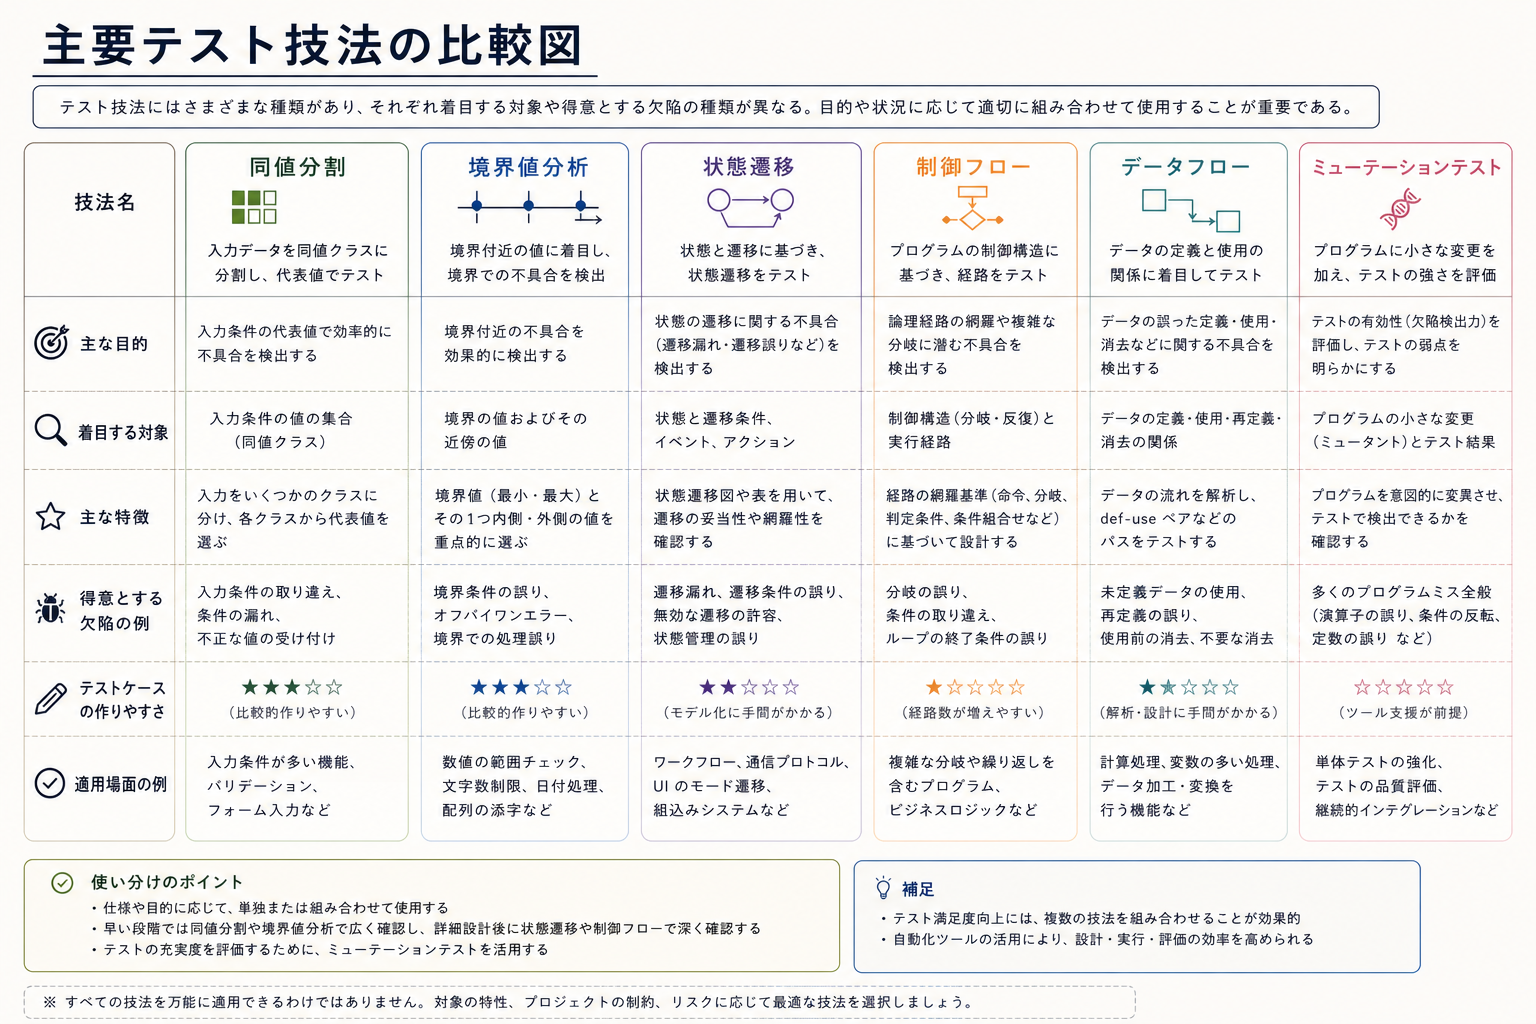
\includegraphics[width=0.96\linewidth]{assets/generated_figures/ch05/fig-ch05-06.png}}{\fbox{\parbox[c][48mm][c]{0.9\linewidth}{\centering 画像生成待ち\\主要テスト技法の比較図}}}
\caption{主要テスト技法の比較図}
\label{fig:ch05-06}
\end{figure}
